\newpage
\subsubsection{Caso d'uso UC4.3: Login tramite Twitter }
\label{UC4_3}
\begin{figure}[!htbp]
	\centering
	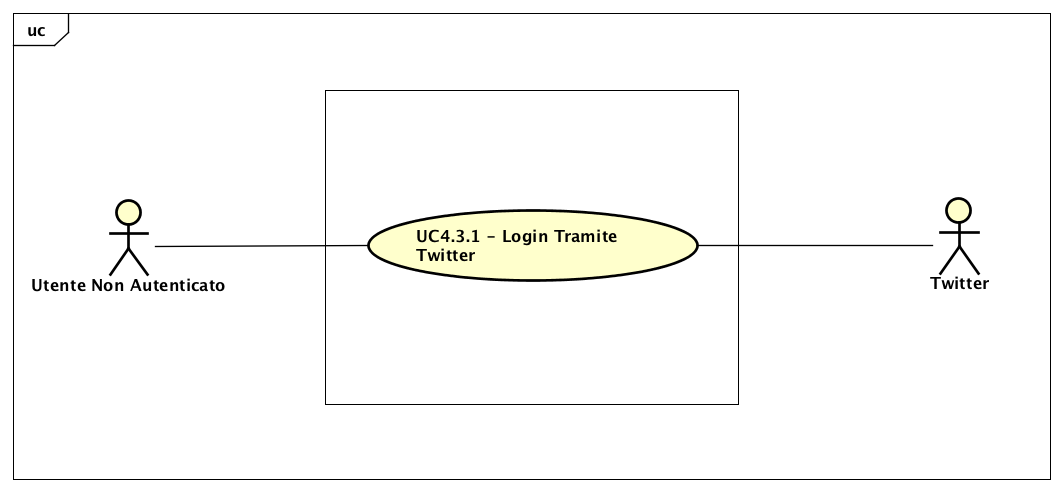
\includegraphics[scale=0.45]{UML/UC4_3.png}
	\caption{UC4.3: Login tramite Twitter}
\end{figure}

\begin{tabular}{ l | p{11cm}}
	\hline
	\rowcolor{Gray}
	\multicolumn{2}{c}{UC4.3 - Login tramite Twitter} \\
	\hline
	\textbf{Attori} & Utente non autenticato, Twitter \\
	\textbf{Descrizione} & L'attore effettua il login all'applicazione web tramite Twitter, così da evolversi in un utente autenticato \\
	\textbf{Pre-Condizioni} & L'attore ha scelto di eseguire il login all'applicazione web tramite Twitter (e non è autenticato) \\
	\textbf{Post-Condizioni} & L'attore ha effettuato il login all'applicazione web tramite Twitter, evolvendosi in un utente autenticato \\
	\textbf{Scenario Principale} & 
	\begin{enumerate*}[label=(\arabic*.),itemjoin={\newline}]
		\item L'attore può effettuare con successo il login tramite Twitter (UC4.3.1), visualizzando un messaggio di successo, e venendo reindirizzato alla pagina principale evolvendosi in un utente autenticato (UC2)
	\end{enumerate*}\\
	\textbf{Scenari Alternativi} & 
	\begin{enumerate*}[label=(\arabic*.),itemjoin={\newline}]
	\item L'attore ha fallito il login tramite Twitter (E.g: Mancanza di privilegi/autorizzazioni, problemi legati a Twitter...) e visualizza un messaggio d'errore (UC4.3.2)
	\end{enumerate*}\\
\end{tabular}